\documentclass[aspectratio=169]{beamer}
\usepackage{basileabeam}
\usepackage{epigraph}
\usepackage{graphicx}

%notes
%\pgfpagesuselayout{2 on 1}[a4paper,border shrink=5mm]
%\setbeamertemplate{note page}[plain]
%\setbeameroption{show notes on second screen=bottom}

\title              {Análise dos modos, efeitos e criticidade de falhas}
\author             {Marco Reis}
\email              {marcoreis@me.com}
\institute          {Laboratório de Robótica e Sistemas Autônomos, Senai Cimatec}
\date               {Abril de 2020}
\ulogo        		{Template/logosenaicimatec}
\ulogoo        		{Template/fibonacci}
\ulistelement    	{Template/sunflower}

\graphicspath{{Figures/}}

\totalNoSlidesDisabled % To turn off the total number of slides in the footer. Comment this if you want the total number of slides in the footer

\begin{document}
%*----------- COVER ------------------------------------------------------------
\begin{frame}[t,plain]
    \titlepage
\end{frame}
%-
\note{Notes can help you to remember important information. Turn on the notes option.}
%*----------- SLIDE ------------------------------------------------------------
\begin{frame}[t]{Introdução} 
%! esta figura tem que sair daqui
A técnica é conhecida como FMECA (\textit{Failure Mode and Effect Criticality Analysis}).

A análise dos modos de falhas, efeitos e criticidade é uma técnica que oferece três funções distintas:
\newline
    \begin{columns}[c]
        \column{.05\textwidth}
        \column{.6\textwidth}
            \begin{enumerate}
                \item ferramenta para prognóstico de problemas
                \item procedimento para desenvolvimento e execução de projetos, processos ou serviços (novos ou revisados)
                \item diário do projeto, processo ou serviço
            \end{enumerate}
        \column{.35\textwidth}
            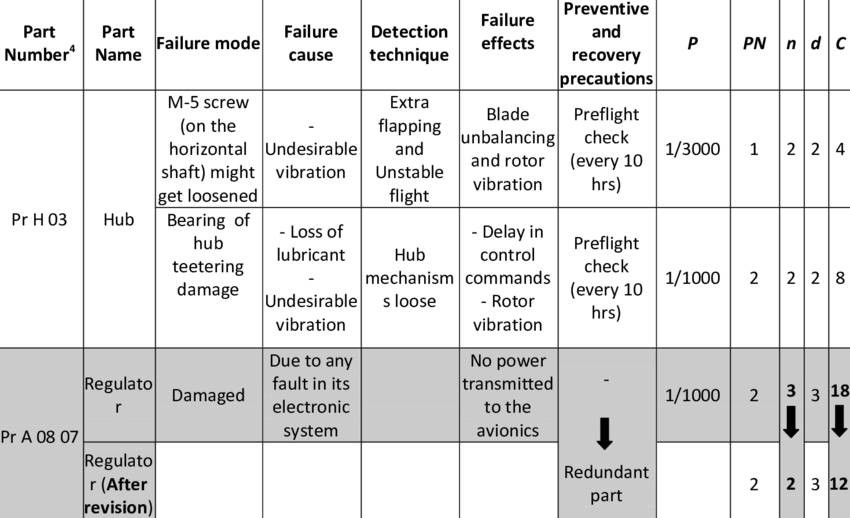
\includegraphics[width=.9\textwidth]{fmeca}
    \end{columns}
\end{frame}
%-
\note{Notes can help you to remember important information. Turn on the notes option.}
%*----------- SLIDE ------------------------------------------------------------
\begin{frame}[t]{FMECA}
    A elaboração da FMECA é muito eficaz quando elaborado em equipe.

    É um método sistemático para identificar e prevenir problemas potenciais.

    Inicialmente, é importante detalhar o sistema em análise apontando os seus subsistemas e componentes.
    
    \setlength\epigraphwidth{.7\textwidth}
    \epigraph{Uma pessoa fazendo o seu melhor, não consegue ser tão eficiente quanto uma equipe trabalhando em conjunto.}{\textit{Marco Reis}}

    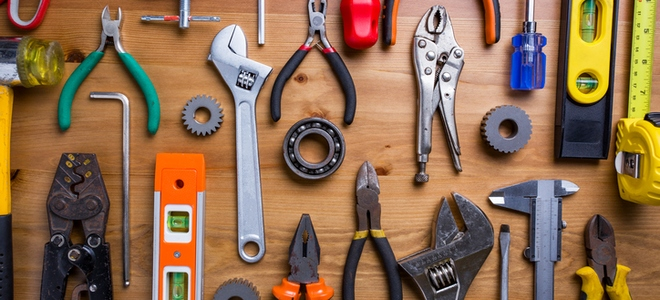
\includegraphics[width=1\textwidth, trim={0 1.8cm 0 0},clip]{tools}
    \raggedleft
\end{frame}
%-
\note{Notes can help you to remember important information. Turn on the notes option.}
%*----------- SLIDE ------------------------------------------------------------
\begin{frame}[t]{Duas Perguntas}
    Quando o foco é o desenvolvimento de um projeto, duas perguntas diretivas devem ser realizadas.
    \newline
    \begin{itemize}
        \item Como esse projeto pode deixar de fazer o que deve fazer?
        \item O que devemos fazer para prevenir essas falhas potenciais de projeto?
    \end{itemize}
    \hfill

    Principais objetivos de uma FMECA:
    \newline
    \begin{columns}[t]
        \column{.45\textwidth}
            detalhar sistemas em subconjuntos\\
            listar possíveis modos de falhas\\
            analisar cada modo de falha, juntamente com suas possíveis causas e sintomas
        \column{.45\textwidth}
            estimar os efeitos de cada modo de falhas\\
            estimar a criticidade de cada efeito\\
            identificar ações para minimizar falhas
    \end{columns}
\end{frame}

%-
\note{Notes can help you to remember important information. Turn on the notes option.}
%*----------- SLIDE ------------------------------------------------------------
\begin{frame}[c]{Some Equations}
Now we introduce an equation.
    \begin{theorem}
    A Turing Machine is a 7-Tuple:
        \begin{equation}
        \label{eq:turi}
            M = \langle Q, \Gamma, b, \Sigma, \delta, q_0, F \rangle
        \end{equation}
    \end{theorem}
A Turing Machine is a 7-Tuple even if defined in the text, as in $M = \langle Q, \Gamma, b, \Sigma, \delta, q_0, F \rangle$.
\end{frame}
%-
\note{Notes can help you to remember important information. Turn on the notes option.}
%*----------- SLIDE ------------------------------------------------------------
\begin{frame}[t]{Items and Numbers}
    \begin{columns}
        \column{.5\textwidth}
            \begin{itemize}
                \item one
                \item two
                \item three
            \end{itemize}
        \column{.5\textwidth}
            \begin{enumerate}
                \item first
                \item second
                \item third
            \end{enumerate}
    \end{columns}
\end{frame}
%-
\note{Notes can help you to remember important information. Turn on the notes option.}
%*----------- SLIDE ------------------------------------------------------------
\begin{frame}[c]{Tables}
Tables are also interesting.
    \begin{table}[ht!]
    \centering
        \begin{tabular}{|l|c|l|} \hline
            Title&$f$&Comments\\ \hline
            The chemical basis of morphogenesis & 7327 & \\ \hline
            On computable numbers & 6347 & Turing Machine\\ \hline
            Computing machinery and intelligence & 6130 & \\ \hline
        \end{tabular}
    \end{table}
\end{frame}
%-
\note{Notes can help you to remember important information. Turn on the notes option.}
%*----------- SLIDE ------------------------------------------------------------
\begin{frame}[c]{Speaker Notes}
You may turn on the notes and handout option to see the notes to the slides.
\end{frame}
%-
\note{Notes can help you to remember important information. Turn on the notes option.}
%----------- BACKUP -----------------------------------------------------------
\backupbegin
%----------- SLIDE ------------------------------------------------------------
\begin{frame}{Backup}
Test
\end{frame}
%-
\note{Notes can help you to remember important information. Turn on the notes option.}

\backupend
%*----------- QUESTIONS --------------------------------------------------------
\begin{frame}[t,plain]
\lastpage{{\usebeamerfont{title} Questions?}\\[3ex] \hspace{0.1cm} marcoreis@me.com}
\end{frame}
%-
\note{Notes can help you to remember important information. Turn on the notes option.}
%*--------------------------------------------------------------------- END-----
\end{document}

